\documentclass[11pt]{article}
\usepackage[letterpaper,margin=1in,headheight=14pt]{geometry}
\usepackage[T1]{fontenc}
\usepackage{lmodern,microtype}
\usepackage{amsmath,amssymb,amsthm,mathtools,booktabs}
\usepackage{graphicx,caption,float,placeins}
\usepackage[hidelinks]{hyperref}
\captionsetup{font=small,labelfont=bf,skip=6pt}
\setlength{\parindent}{1em}
\setlength{\parskip}{0pt}
\setlength{\textfloatsep}{14pt}
\setlength{\intextsep}{12pt}
\renewcommand{\topfraction}{0.90}
\renewcommand{\bottomfraction}{0.90}
\renewcommand{\textfraction}{0.08}
\renewcommand{\floatpagefraction}{0.75}
\setcounter{topnumber}{3}
\setcounter{totalnumber}{4}
\emergencystretch=1.5em
\graphicspath{{figures/}}
\hypersetup{pdftitle={From the original link function to surface envelopes},pdfauthor={Research meeting report}}
\title{From the Original Link Function to Surface Envelopes}
\author{Research meeting report}
\date{September 2026}
\begin{document}
\begin{center}
{\Large\bfseries From the Original Link Function to Surface Envelopes\par}
\vspace{0.7em}
Research meeting report\qquad September 2026
\end{center}
\vspace{0.4em}
\begin{abstract}
We revisit the original transductive link function, its small extension to
signed residuals, global worst-case calibration, and the full local worst-case
construction. The surface envelope replaces separated location and scale
bounds by an exact supremum of their ratio. We give its construction and prove
that, on identical nonnegative residuals, it produces a weakly smaller valid
rectangle than the original shortcut. Focused paired experiments examine
calibration size, miscoverage, and prediction-set geometry. A separate signed
quantile-residual comparison gives the old method capped and two valid shifted
representations, including a width-dependent shift that preserves all score
information. All displayed data, code, figures, and source files accompany
this report in one folder.
\end{abstract}

\newtheorem{mtproposition}{Proposition}
\newtheorem{mttheorem}{Theorem}

\section{The original link function, including signed residuals}
Condition on a predictor fitted independently of the calibration and test data.
Let $\mathbf E^1,\ldots,\mathbf E^{n+1}\in\mathbb R^d$ be exchangeable
coordinatewise residual vectors, with the first $n$ observed. Write $N=n+1$,
$r=\lceil N(1-\alpha)\rceil$, and
\[
 Q_\alpha(v_1,\ldots,v_n)=v_{(r)}\quad(r\le n),
 \qquad Q_\alpha(v_1,\ldots,v_n)=+\infty\quad(r=N).
\]
Throughout, acceptance uses weak inequalities. Ties are permitted. Define
the calibration statistics $m_j=n^{-1}\sum_i E^i_j$ and
$s_j^2=n^{-1}\sum_i(E^i_j-m_j)^2$, initially with every $s_j>0$.
The original paper \cite{fan2025} augments these observations with a candidate residual
$z_j$ and uses
\begin{equation}\label{mt:augmented}
 \mu_j(z)=\frac{nm_j+z}{N},\qquad
 \sigma_j(z)=\sqrt{s_j^2+\frac{(z-m_j)^2}{N}},\qquad
 F_j(t,z)=\frac{t-\mu_j(z)}{\sigma_j(z)}.
\end{equation}
Here $s_j^2$ has divisor $n$, whereas the augmented sample variance has
divisor $N-1=n$. The distinction determines the constants below.
The candidate's self-score and scalarized calibration score are
\begin{equation}\label{mt:self}
 g_j(e)=F_j(e,e)=
 \frac{n(e-m_j)/N}{\sqrt{s_j^2+(e-m_j)^2/N}},\qquad
 \Phi_{\mathbf z}(\mathbf t)=\max_jF_j(t_j,z_j).
\end{equation}

The original nonnegative link has a positive middle branch
$m_j+Ns_j|c|/\sqrt{n^2-Nc^2}$, a negative middle branch
$\max\{0,m_j-Ns_j|c|/\sqrt{n^2-Nc^2}\}$, and outer values zero and
$+\infty$ at $c\le-n/\sqrt N$ and $c\ge n/\sqrt N$.
Its algebra already supports signed residuals: remove the truncation at zero,
preserve the sign of the middle root, and represent an empty lower branch by
$-\infty$. The resulting exact inverse is
\begin{equation}\label{mt:link}
 \omega_j(c)=\begin{cases}
 -\infty,&c\le -T,\\[2pt]
 m_j+\displaystyle\frac{Ns_jc}{\sqrt{n^2-Nc^2}},&-T<c<T,\\[5pt]
 +\infty,&c\ge T,
 \end{cases}\qquad T=\frac n{\sqrt N}.
\end{equation}
Indeed, $g_j'(e)=(n/N)s_j^2\{s_j^2+(e-m_j)^2/N\}^{-3/2}>0$,
its range is $(-T,T)$, and solving $g_j(e)=c$ requires
$\operatorname{sign}(e-m_j)=\operatorname{sign}(c)$. Hence, for finite $e$,
\begin{equation}\label{mt:inverse}
 g_j(e)\le c\quad\Longleftrightarrow\quad e\le\omega_j(c).
\end{equation}
For nonnegative scores one intersects this sublevel with $[0,\infty)$;
for signed scores one uses the appropriate attainable domain. Clamping a
negative endpoint to zero would turn an empty sublevel into a singleton, so
the unclamped form is useful even for a precise treatment of nonnegative ties.

At test input $x$, suppose $E_j(x,y_j)$ takes values in
$D_j(x)=[a_j(x),\infty)\cap\mathbb R$, allowing $a_j=-\infty$.
For absolute residuals, $E_j=|y_j-\hat f_j(x)|$ and $a_j=0$.
For signed CQR residuals \cite{romano2019}, with ordered fitted quantiles,
\begin{align}\label{mt:cqr}
 E_j(x,y_j)&=\max\{\hat q_j^-(x)-y_j,\ y_j-\hat q_j^+(x)\}
             =|y_j-\hat m_j(x)|-h_j(x),\notag\\
 \hat m_j(x)&=\tfrac12(\hat q_j^-+\hat q_j^+),\qquad
 h_j(x)=\tfrac12(\hat q_j^+-\hat q_j^-),\qquad a_j(x)=-h_j(x).
\end{align}
Thus a threshold $L_j$ gives $[\hat q_j^- - L_j,\hat q_j^+ + L_j]$;
negative thresholds shrink the fitted interval. The domain lower bound is
known from the fitted interval at $x$, and is not a minimum estimated from
the calibration scores. Those scores, observed at other inputs, may lie below
$a_j(x)$. The link is therefore not the obstacle to signed residuals; the
nonnegative scale separation in the old shortcut is.

\section{Review: GWC, full LWC, and the old shortcut}
\paragraph{Full conformal reference and GWC.}
For a candidate $\mathbf e=\mathbf E(x,y)$ define
\[
 q(\mathbf e)=Q_\alpha\bigl(\Phi_{\mathbf e}(\mathbf E^1),\ldots,
                                  \Phi_{\mathbf e}(\mathbf E^n)\bigr),\qquad
 C_{\rm full}(x)=\{y:\max_jg_j(e_j)\le q(\mathbf e)\}.
\]
This candidate-dependent set is the reference we enclose, and need not be
rectangular. For an interval $I$ put
$\psi_{j,I}(t)=\sup_{z\in I}F_j(t,z)$. GWC uses
\begin{equation}\label{mt:gwc}
 \Phi_G(\mathbf t)=\max_j\psi_{j,D_j(x)}(t_j),\quad
 q_G=Q_\alpha\bigl(\Phi_G(\mathbf E^i):i\le n\bigr),\quad
 U_j=\omega_j(q_G),\quad G_j=D_j(x)\cap(-\infty,U_j].
\end{equation}
Every candidate in $D(x)=\prod_jD_j(x)$ has $q(\mathbf e)\le q_G$;
hence $C_{\rm full}(x)\subseteq\{y:\mathbf E(x,y)\in G\}$, where
$G=\prod_jG_j$. This reviews the original GWC when $D_j=[0,\infty)$
and extends the same construction to signed scores.

\paragraph{The original full LWC.}
For nonnegative residuals, partition each $G_j=[0,U_j]$ at its interior
calibration residuals. We use closed cells
$I_{j,k}=[\eta_{j,k-1},\eta_{j,k}]\cap\mathbb R$ so shared boundary points
are retained. A full cell is $\mathcal I_{\mathbf h}=\prod_jI_{j,h_j}$;
there are at most $(n+1)^d$ such cells. The original paper uses
\begin{equation}\label{mt:separated}
 c_j=\inf_{z\in G_j}\frac{\mu_j(z)}{\sigma_j(z)},\qquad
 r_j(k)=\inf_{z\in I_{j,k}}\sigma_j(z),\qquad
 \Phi^{\rm sep}_{\mathbf h}(\mathbf t)
       =\max_j\left\{\frac{t_j}{r_j(h_j)}-c_j\right\},\quad\mathbf t\ge0.
\end{equation}
Its cell quantile $q^{\rm sep}_{\mathbf h}=Q_\alpha(
\Phi^{\rm sep}_{\mathbf h}(\mathbf E^i):i\le n)$ produces the local region
\[
 R^{\rm sep}_{\mathbf h}=
 \mathcal I_{\mathbf h}\cap\prod_j(-\infty,\omega_j(q^{\rm sep}_{\mathbf h})].
\]
Full LWC enumerates these regions, takes their union, and reports its
coordinatewise upper enclosure within $G$. This is a local bound on the
unknown candidate, followed by a rectangular enclosure; it is not full
conformal prediction itself.

For clarity, an \emph{exact coupled} full-cell alternative would replace
$\Phi^{\rm sep}_{\mathbf h}$ by
$\Phi^{\rm exact}_{\mathbf h}(\mathbf t)=
\max_j\psi_{j,I_{j,h_j}}(t_j)$.
It retains the whole ratio under each supremum and is no larger than the
separated cell score for nonnegative $\mathbf t$. It is a sharper conceptual
reference, not the separated full LWC defined in the original paper.
Neither full-cell construction is run in the meeting experiments.

\paragraph{The old row shortcut.}
The paper avoids enumerating all cells by varying one coordinate at a time,
holding the others in a cell containing the empirical mean. If GWC clips that
cell, the relevant point is $p_\ell=\operatorname{proj}_{G_\ell}(m_\ell)$,
with $\bar s_\ell=\sigma_\ell(p_\ell)$, the minimum scale on $G_\ell$.
The row score for coordinate $j$ and cell $k$ is
\begin{equation}\label{mt:oldrow}
 \Phi^{\rm old}_{j,k}(\mathbf t)=
 \max\left\{\frac{t_j}{r_j(k)}-c_j,
             \max_{\ell\ne j}\left(\frac{t_\ell}{\bar s_\ell}-c_\ell\right)
      \right\}.
\end{equation}
Its quantile, inverse link, and intersection with $I_{j,k}$ determine a
candidate upper endpoint; maximizing over $k$ gives $L_j^{\rm old}$.
The manuscript's row reduction applies under its mean-cell condition, and
the implemented shortcut falls back to GWC if this cell is unavailable.
The old shortcut here means this separated row construction with compatible
weak boundary conventions. Its key restriction is $t_\ell\ge0$:
$t_\ell/\sigma_\ell(z)\le t_\ell/\inf\sigma_\ell$ reverses for negative
$t_\ell$. Simply changing the inverse link cannot repair that inequality.

\section{The envelope construction}
\paragraph{An exact, inexpensive coordinate bound.}
Unlike scale separation, $\psi_{j,I}(t)$ is valid for either sign of $t$.
Suppressing $j$ and writing $I=[\ell,u]\cap\mathbb R$, differentiation gives
\begin{equation}\label{mt:derivative}
 \frac{\partial F(t,z)}{\partial z}
 =-\frac{s^2+(t-m)(z-m)}{N\{s^2+(z-m)^2/N\}^{3/2}}.
\end{equation}
For $t>m$, the sole stationary maximum is
$z^*(t)=m-s^2/(t-m)$, with value
$\sqrt{(t-m)^2/s^2+1/N}$. For $t<m$ the stationary point is a minimum,
and for $t=m$ the function is decreasing. Therefore
\begin{equation}\label{mt:supremum}
 \psi_{j,I}(t)=\max\left\{
 F_j(t,\ell),F_j(t,u),
 \left.\sqrt{(t-m_j)^2/s_j^2+1/N}\ \right|\ t>m_j,\ z^*(t)\in I
 \right\}.
\end{equation}
The last entry is omitted if inadmissible. Infinite endpoints use
$F_j(t,-\infty)=1/\sqrt N$ and $F_j(t,+\infty)=-1/\sqrt N$.
This formula computes all GWC and envelope scores without numerical optimization.

\paragraph{One coordinate cell, with the others bounded globally.}
Build GWC using \eqref{mt:gwc}, now with either residual domain. Subdivide
each nonempty $G_j$ at its distinct interior calibration values, retaining
singletons when necessary. For each $j$, precompute
\begin{align}\label{mt:surface}
 H_j(\mathbf t)&=\max_{\ell\ne j}\psi_{\ell,G_\ell}(t_\ell),\notag\\
 \overline\Phi_{j,k}(\mathbf t)
  &=\max\{\psi_{j,I_{j,k}}(t_j),H_j(\mathbf t)\}
   =\sup_{\substack{z_j\in I_{j,k}\\z_\ell\in G_\ell,\ \ell\ne j}}
      \Phi_{\mathbf z}(\mathbf t),\notag\\
 \overline q_{j,k}&=Q_\alpha\bigl(\overline\Phi_{j,k}(\mathbf E^i):i\le n\bigr).
\end{align}
For $d=1$, set $H_1=-\infty$. Thus the envelope keeps one coordinate local
and lets all other candidate coordinates range over GWC. It retains the
coupled location--scale ratio while replacing exponential full-cell
enumeration by coordinate searches. Define
\begin{align}\label{mt:pieces}
 A_{j,k}&=I_{j,k}\cap(-\infty,\omega_j(\overline q_{j,k})],\qquad
 L_j=\max_k B_{j,k},\notag\\
 B_{j,k}&=\begin{cases}
 \min\{\eta_{j,k},\omega_j(\overline q_{j,k})\},&A_{j,k}\ne\varnothing,\\
 -\infty,&A_{j,k}=\varnothing,
 \end{cases}
\end{align}
The final region is
$C_{\rm env}(x)=\{y:E_j(x,y_j)\in D_j(x),\ E_j(x,y_j)\le L_j\ \forall j\}$.
It is empty if any coordinate has no accepted piece. It can fill gaps between
pieces, and generally differs from both full conformal and full-cell LWC.
For ordinary absolute or CQR residuals, its outcome sublevels are intervals,
so the final region is a box.

\paragraph{Search and cost.}
With the calibration coordinates sorted, scan cells from right to left and
stop at the first nonempty piece. This is exact: every earlier cell ends at
or below the surviving cell's left endpoint, and therefore cannot give a
larger $B_{j,k}$. No unproved monotonicity of acceptance is required.
All off-coordinate values $H_j(\mathbf E^i)$ can be precomputed in $O(nd)$
using prefix and suffix maxima. Each inspected cell then costs $O(n)$ with
order-statistic selection. Total worst-case cost is
$O(dn\log n+dn^2)$, and actual search cost is $O(n\sum_j M_j)$ when
$M_j$ cells are inspected. This establishes tractability, not uniform runtime
dominance. Calibration statistics can be reused; input-dependent CQR widths
may require different domain calculations at different test inputs.

\section{Validity and uniform improvement: separate proofs}
\begin{mtproposition}[Finite-sample validity]\label{mt:validity}
For every realized positive-scale calibration sample and test input,
$C_{\rm full}(x)\subseteq C_{\rm env}(x)\subseteq C_{\rm GWC}(x)$.
Under exchangeability, $\Pr\{Y^{n+1}\in C_{\rm env}(X^{n+1})\}\ge1-\alpha$.
\end{mtproposition}
\begin{proof}
At the true test residual, the augmented means and scales are symmetric
functions of all $N$ observations. Applying the same standardized maximum
to all observations gives exchangeable scalar scores. The conformal rank
argument, including weak acceptance for ties, gives coverage at least
$r/N\ge1-\alpha$ for $C_{\rm full}$.

For an accepted candidate $\mathbf e$, GWC containment gives $\mathbf e\in G$.
Choose for each $j$ a covering cell $I_{j,k}$ containing $e_j$.
Every calibration score obeys
$\Phi_{\mathbf e}(\mathbf E^i)\le\overline\Phi_{j,k}(\mathbf E^i)$.
Coordinatewise ordering of a score vector preserves ordering of its $r$th
order statistic; hence $q(\mathbf e)\le\overline q_{j,k}$.
Full acceptance and the increasing link imply
$e_j\le\omega_j(\overline q_{j,k})$, so $e_j\in A_{j,k}$ and $e_j\le L_j$.
This holds for every coordinate without a Bonferroni adjustment.
Finally, every piece lies in $G_j$, giving $L_j\le U_j$.
\end{proof}

\begin{mttheorem}[Uniform weak improvement over the old shortcut]\label{mt:dominance}
Use the same nonnegative residuals, calibration sample, $\alpha$, GWC domain,
and closed cells for both methods, with $s_j>0$. Then
\[
 C_{\rm env}(x)\subseteq C_{\rm old}(x).
\]
For nonempty regions this means $L_j\le L_j^{\rm old}$ in every coordinate,
and therefore weakly smaller outcome intervals and volume. Envelope coverage
remains at least $1-\alpha$.
\end{mttheorem}
\begin{proof}
For $t_j\ge0$ and $z\in I_{j,k}$,
\[
 F_j(t_j,z)=\frac{t_j}{\sigma_j(z)}-\frac{\mu_j(z)}{\sigma_j(z)}
 \le\frac{t_j}{r_j(k)}-c_j.
\]
For an off-coordinate $\ell$, the same inequality on $G_\ell$ gives
$\psi_{\ell,G_\ell}(t_\ell)\le t_\ell/\bar s_\ell-c_\ell$.
Consequently $\overline\Phi_{j,k}(\mathbf E^i)\le
\Phi^{\rm old}_{j,k}(\mathbf E^i)$ for every $i,j,k$.
Quantile monotonicity and \eqref{mt:inverse} imply that every envelope piece
is contained in the corresponding old piece. Taking upper endpoints and
then maxima proves the result. If the old shortcut falls back to GWC,
Proposition~\ref{mt:validity} gives containment directly.
\end{proof}

The separation bound can be strict because the smallest scale and smallest
location--scale ratio occur at different candidate values. For a concrete
one-dimensional example, take calibration residuals $(1,2,3)$ and
$\alpha=1/2$. Then $m=2$, $s^2=2/3$, $r=2$, and GWC ends at
$U=2+2/\sqrt{21}$. On $[2,U]$, the envelope's median score is zero,
so $L^{\rm env}=2$; the separated median is
$\sqrt6-\sqrt{27/20}$, whose link exceeds $U$, so $L^{\rm old}=U$.
The absolute-residual interval is strictly shorter. Equality is also
possible, for example when $r=N$ and both methods return the whole domain.
The theorem does not assert strict improvement on every sample, higher
coverage than a superset, or dominance over exact coupled full-cell LWC.

\paragraph{Scope of the signed comparison.}
Capping $E$ at zero loses negative values; shifting by a width that changes
with $x$ changes relative residuals across observations. The preceding theorem
does not compare those representations. A fixed coordinatewise shift has
additional structure: if a training-only constant $b_j$ satisfies
$E_j(x,y)\ge-b_j$ everywhere, then
$F_j^{\rm shift}(t+b_j,z+b_j)=F_j(t,z)$ and
$\omega_j^{\rm shift}(c)=\omega_j(c)+b_j$.
The signed attainable domain translates into a subset of $[0,\infty)$.
Taking suprema on that smaller domain and applying the same proof shows that
the signed envelope is contained in the old constant-shifted region, under
matching exact boundary rules. No analogous containment is claimed against
capping or input-dependent width shifts; their practical comparison is empirical.

\paragraph{Boundary and implementation conventions.}
If $r=N$, return the whole attainable domain. If any observed $s_j=0$, the
experiments use a common whole-domain fallback; the displayed dominance proof
concerns positive scales. A valid full-conformal reference on degenerate
samples uses augmented scale $1$ when that entire augmented coordinate is
constant; this symmetric rule and the whole-domain fallback preserve coverage.
Closed cells retain singleton endpoints. Mathematical inequalities refer to
exact arithmetic with these conventions; the old executable's numerical
jitter and finite-precision outputs are checked separately. All coverage
statements average over calibration and test data, rather than asserting
coverage conditional on a particular input or calibration sample.

\section{Absolute residuals: controlled paired comparisons}
\label{sec:absolute}

\paragraph{Data generation and fitted prediction rule.}
Each trial independently draws 800 training observations, $n$ calibration
observations, and 1,200 test observations. Let $X\sim N(0,I_3)$,
$g(X)=\mathbf 1\{X_1>0\}$, and, for $j=1,\ldots,d$,
\begin{equation}\label{eq:toy-model}
 Y_j=X^\top\beta_j+(1+0.8g(X))\tau_j\varepsilon_j,
 \quad \beta_{kj}=\tfrac12\sin\{(k-1)d+j\},\quad
 \tau_j=0.6\,4^{(j-1)/(d-1)}.
\end{equation}
The four noise laws have zero mean and unit variance: independent Gaussian;
Gaussian with equicorrelation $0.8$; independent Laplace with scale
$1/\sqrt2$; and independent standardized lognormal,
$\varepsilon_j=(e^{0.8Z_j}-e^{0.32})/
\sqrt{(e^{0.64}-1)e^{0.64}}$ with $Z_j\sim N(0,1)$.
An OLS model with intercept is fitted on training observations only. Both
methods use the same absolute residuals
$E_j(x,y_j)=|y_j-\widehat f_j(x)|$, calibration data, and test observations.
Thus any difference in this section comes from calibration, not refitting
or changing the residual definition. A threshold vector $L$ gives
$\prod_j[\widehat f_j(x)-L_j,\widehat f_j(x)+L_j]$ with volume
$2^d\prod_jL_j$.

\paragraph{Scope and uncertainty.}
The calibration-size study uses $d=6$, $\alpha=0.1$, $n\in\{30,80,200\}$,
four noise laws, and 120 independent fitted trials per setting (1,440 total).
The target study keeps $d=6,n=80$ and uses Gaussian and Laplace noise at
$\alpha\in\{0.05,0.1,0.2,0.3\}$; the $0.1$ results are the same trials as
in the first study. There are 2,160 distinct absolute-score trials overall.
These are retained independent fitted trials from the earlier report, with
both methods rerun from the saved scores for this revision; they are not
new independent replications of that evidence.

Joint coverage is the fraction of test observations inside all coordinate
intervals. Size comparisons average the \emph{within-trial} volume ratio
$V_{\rm env}/V_{\rm old}$, not a ratio of pooled means. Error bars are
pointwise 95\% Student-$t$ Monte Carlo intervals across the 120 trial values.
Test observations within one fitted trial are not treated as independent
replications for these error bars. All absolute regions here are finite.
The old implementation retains its original deterministic $10^{-10}$ score
jitter; the mathematical theorem uses closed cells without jitter. The
reported numerical checks use a relative endpoint tolerance of $10^{-8}$.

\begin{figure}[tbp]
\centering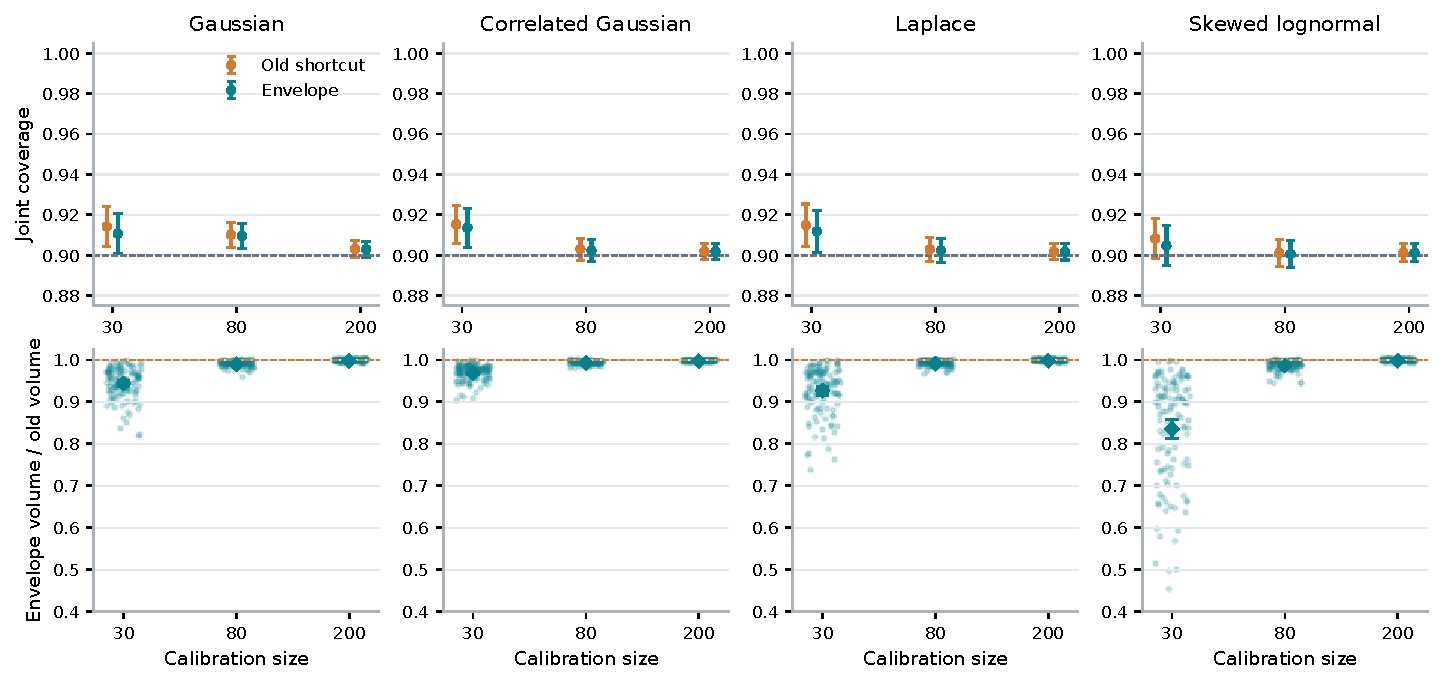
\includegraphics[width=\linewidth]{absolute_n.pdf}
\caption{Calibration-size comparison on identical absolute residuals.
Top: joint coverage, with target $0.9$ dashed. Bottom: paired volume ratios;
faint points are individual fitted trials, diamonds are means, and bars are
95\% Monte Carlo intervals. Each setting has 120 trials, $d=6$.}
\label{fig:absolute-n}
\end{figure}

\paragraph{Calibration size: the strongest gains occur with limited data.}
At $n=30$, the mean paired volume reductions are 5.64\% (Gaussian),
3.11\% (correlated Gaussian), 7.36\% (Laplace), and 16.44\% (skewed
lognormal). Their 95\% Monte Carlo half-widths are respectively 0.67,
0.34, 1.01, and 2.32 percentage points. At $n=80$ the reductions narrow
to 0.77--1.37\%; at $n=200$ they are 0.23--0.34\%.
The envelope therefore offers a distribution-free direction of improvement,
but its magnitude is strongly setting dependent. The skewed, small-sample
case is the clearest empirical gain in this grid.

Across all 2,160 paired trials and 12,960 coordinate comparisons, there are
no containment violations. In the size study, envelope mean joint coverage
ranges from 0.9006 to 0.9135 and stays close to the 0.9 target. It is slightly
lower than old-shortcut coverage, as nesting requires; shrinking a conservative
region is the intended efficiency gain. The experiment supports the theorem
but does not substitute for it.

\paragraph{Different target levels.}
At $n=80$, paired volume reductions span 1.05--1.64\% for Gaussian noise
and 0.85--1.85\% for Laplace across the four targets. The largest reductions
in both families occur at $\alpha=0.05$, but the curves are not generally
monotone in $\alpha$. Mean envelope coverage exceeds its nominal target by
0.03--1.15 percentage points across these settings. Thus the refinement
persists across targets without a universal claim about how its magnitude
must change with $\alpha$.


\begin{figure}[tbp]
\centering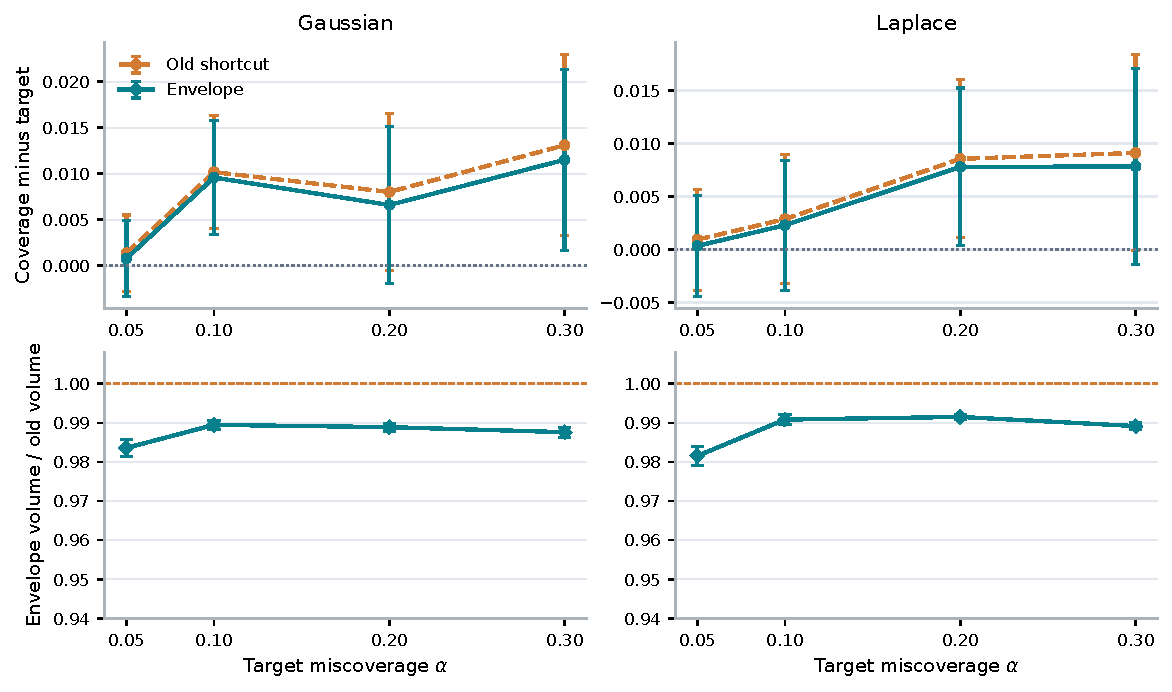
\includegraphics[width=0.88\linewidth]{absolute_alpha.pdf}
\caption{Miscoverage sensitivity at $n=80,d=6$, 120 fitted trials per point.
Top: coverage minus $1-\alpha$ (zero is nominal). Bottom: paired volume ratio.
Error bars describe Monte Carlo uncertainty, not a simultaneous coverage test.}
\label{fig:absolute-alpha}
\end{figure}

\paragraph{What the regions look like.}
Figure~\ref{fig:absolute-region} uses a separately generated two-dimensional
Laplace trial, $n=30$, $\alpha=0.1$, seed 2026990918 and test input 0, fixed
before viewing the geometry. The displayed axes subtract the fitted center
and divide by the known DGP scales $\tau_j$, solely for visualization.
The enlargement near the upper-right corner makes a modest boundary change
visible while the main axes preserve its true size. The area ratio is
$0.9750$: a 2.50\% reduction. Gray shading evaluates the full-conformal
acceptance rule on a $301\times301$ grid; every accepted grid point is
inside the envelope. This grid is an illustration, not an exact set-area
calculation or a coverage experiment. Full LWC is reviewed mathematically;
the report does not run its exponential full-cell enumeration.

\begin{figure}[H]
\centering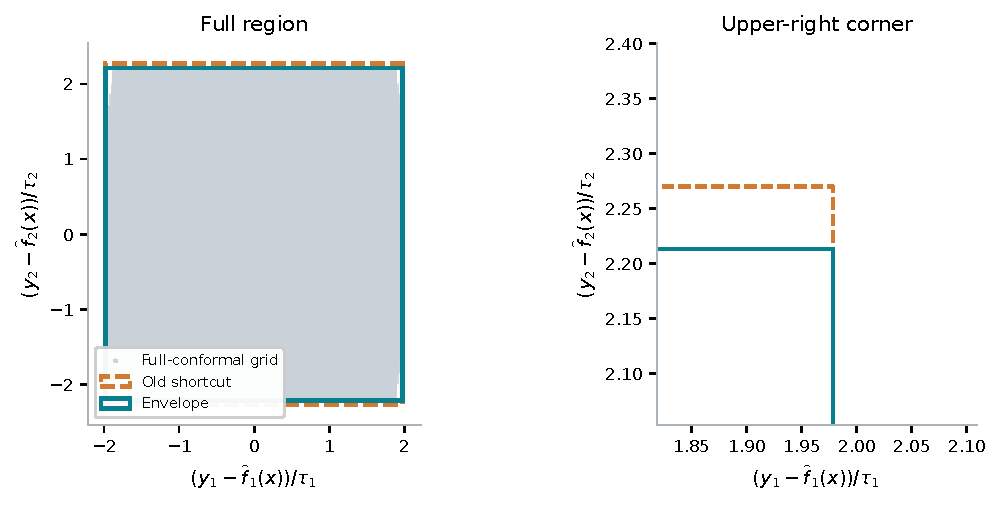
\includegraphics[width=\linewidth]{absolute_region.pdf}
\caption{One fixed-input absolute-residual region. Orange dashed: old
shortcut; teal: envelope; gray: full-conformal grid acceptance. Both axes
use the same coordinate normalization for every method. The right panel shows the
upper-right corner without changing the scale of the main plot.}
\label{fig:absolute-region}
\end{figure}

\section{Signed residuals and strong versions of the old shortcut}
\label{sec:signed-experiments}

The additional benefit here is the ability to use negative residuals directly.
For a fitted base interval $[\ell_j(x),u_j(x)]$, write its midpoint as $m_j(x)$
and half-width as $h_j(x)$. The signed quantile residual is
\[
 r_j(x,y)=\max\{\ell_j(x)-y_j,\,y_j-u_j(x)\}
         =|y_j-m_j(x)|-h_j(x)\geq-h_j(x).
\]
A negative threshold contracts the fitted interval. The envelope uses these
raw scores and the attainable candidate domain $[-h_j(x),\infty)$ directly.
The old shortcut's nonnegative-score construction requires a transformation;
we give it three valid versions, all fixed by the training fit:
\begin{enumerate}
\item \emph{Capping}: use $r_j^+=\max(r_j,0)$. This discards the depth of
  observations inside the base interval and cannot contract the base.
\item \emph{Constant shift}: set $c_j=\max_{g\in\{0,1\}}h_{gj}$ and use
  $r_j+c_j$. This is the smallest constant coordinatewise shift certified by
  the fitted base widths over both covariate groups. Subtract $c_j$ from the
  old threshold when mapping back to the outcome space.
\item \emph{Width shift}: use $r_j(x,y)+h_j(x)=|y_j-m_j(x)|$. Subtract
  $h_j(x)$ from the old threshold at prediction. This is a covariate-dependent
  transformation, rather than a common translation, and is also nonnegative
  for every future observation.
\end{enumerate}
Both shifts preserve the residual value when their known offsets are retained;
neither uses a calibration minimum. In particular, signed support is an
advantage of the new construction, but does not mean the old method has no
valid workaround. No envelope calculation is applied to capped residuals in
these comparisons.

We use three settings, each with 120 paired fitted trials, 800 training
observations, $n=80$ calibration observations, 1,200 test observations and
$\alpha=0.1$. Two settings have Gaussian noise and two outcomes, with fitted
nominal marginal base coverage levels of 90\% and 98\%; the wider base deliberately
tests contraction. The third has Laplace noise and six outcomes with a 90\%
marginal base. The data model and OLS training procedure are the same as in the
absolute-residual experiments. To fit the base intervals, compute training
errors $Y_j-\widehat f_j(X)$ separately in the two groups $g(X)=0,1$.
If $\delta$ is the base miscoverage (0.1 or 0.02), let $a_{gj}^-$ and
$a_{gj}^+$ be their empirical $\delta/2$ and $1-\delta/2$ quantiles.
Then $\ell_j(x)=\widehat f_j(x)+a_{g(x),j}^-$ and
$u_j(x)=\widehat f_j(x)+a_{g(x),j}^+$. These offsets are estimated only
from training data; nominal base coverage need not equal achieved joint
coverage. All four methods receive the same observations
and fitted intervals within a trial. We compare every version separately;
identifying the smallest average old volume below is a descriptive comparison,
not a rule that chooses a method on calibration or test outcomes.
These 360 trials reuse the prior fitted observations; the shifted baselines
are newly evaluated in this revision. The 120 six-output Laplace fits also
appear in the absolute study, so the two sections are paired views of those
fits, not independent additional evidence. For a threshold $L_j(x)$, the
outcome volume is $\prod_j\{2h_j(x)+2L_j(x)\}$ when all coordinate lengths
are nonnegative, and zero if any coordinate interval is empty. Each trial
averages this volume over its 1,200 test inputs before paired ratios are
formed; zero-length singleton intervals have zero volume but are retained.

\begin{figure}[tbp]
\centering

\includegraphics[width=\linewidth]{figures/signed_comparison.pdf}
\caption{Raw signed envelope versus three valid nonnegative versions of the
old shortcut. Top: simultaneous test coverage. Bottom: mean paired outcome
volume ratios, with the named old version as denominator. Bars are pointwise
95\% Monte Carlo intervals across independent fitted trials. All coverage
summaries include infinite regions. Only the wide-base capped comparison
excludes nonfinite volume pairs: 91 of 120 pairs remain; the other 29 capped
regions are infinite. Every other ratio uses all 120 pairs.}
\label{fig:signed-comparison}
\end{figure}

Figure~\ref{fig:signed-comparison} shows why the shifted baselines matter.
With the ordinary 90\% Gaussian base, capping has the smallest average old
volume; the envelope's mean paired volume is $0.42\%$ larger, with a 95\%
interval of $[-0.23\%,1.07\%]$ for this difference. Thus there is no empirical
gain over the strongest old version in this setting. With the 98\% Gaussian
base, old capping is overconservative (coverage $0.9613$, MCSE $0.0022$) and
produces infinite regions in $29/120$ trials under the stated zero-scale
fallback: at least one coordinate has all capped calibration scores equal
to zero. This is a conservative implementation convention, rather than a
claim that every possible treatment of capped ties must be infinite.
The two shifts remove that
problem. The constant shift has the smallest average old volume, and the
envelope reduces the paired volume by $1.79\%\pm0.12\%$ relative to it;
coverage is $0.9071$ (MCSE $0.0026$), versus $0.9114$ (MCSE $0.0025$) for
the constant shift. Negative envelope adjustments occur in 88.7\% of
test-coordinate cases, illustrating contraction of an overly wide base.

For the six-outcome Laplace setting, the envelope's paired volume reduction
is $15.83\%\pm3.89\%$ relative to old capping, but $1.46\%\pm0.20\%$
relative to the stronger constant shift. Their coverages are $0.9049$
(MCSE $0.0031$) and $0.9057$ (MCSE $0.0031$), respectively. These small but
consistent gains against a strong shifted implementation are the relevant
size comparison. Changing to capped or covariate-shifted scores also changes
the conformal construction, so these experiments do not assert a universal
ordering across those score choices.

\begin{figure}[tbp]
\centering
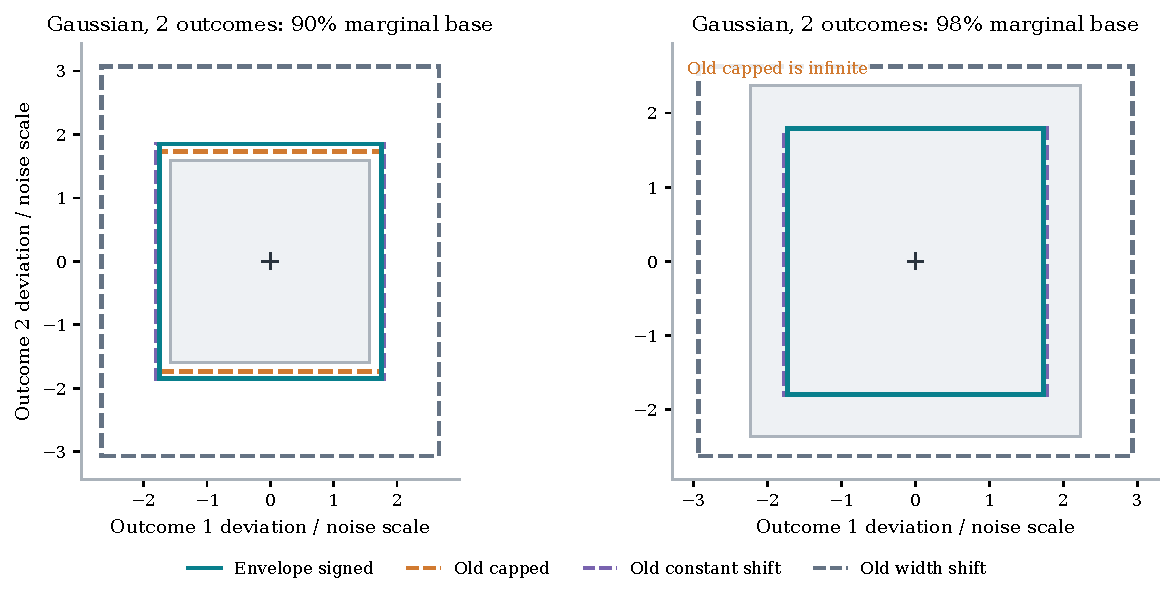
\includegraphics[width=.97\linewidth]{figures/signed_regions.pdf}
\caption{Outcome regions for the two Gaussian settings at predetermined
trial 0 and test observation 0. Axes are deviations from the fitted base
midpoint divided by the coordinate noise scale; the pale rectangle is the
fitted base interval product. The ordinary base need not favor signed
residuals over capping. With the wide base, the signed envelope and the
constant-shifted shortcut both contract it; their size difference is modest.
The width shift is valid but loses the original covariate-dependent base-width
adjustment, which makes its region visibly larger at this observation.
The capped region in the right panel is infinite.}
\label{fig:signed-regions}
\end{figure}

\FloatBarrier
\begin{thebibliography}{9}
\bibitem{fan2025} Yunjie Fan and Matteo Sesia.
Interpretable Multivariate Conformal Prediction with Fast Transductive
Standardization. arXiv:2512.15383, 2025.
\url{https://arxiv.org/abs/2512.15383}.
The notation and the full LWC review follow the working manuscript supplied
with this project; source snapshots are included in \texttt{sources/}.

\bibitem{romano2019} Yaniv Romano, Evan Patterson, and Emmanuel J. Cand\`es.
Conformalized Quantile Regression. \emph{Advances in Neural Information
Processing Systems}, 32, 2019.
\url{https://proceedings.neurips.cc/paper/2019/hash/5103c3584b063c431bd1268e9b5e76fb-Abstract.html}.
\end{thebibliography}
\end{document}
